%\documentclass[12pt]{scrreprt}
\documentclass[12pt]{report} 

% language may be romanian or english (default is english)
% type may be bachelor or master (default is bachelor)
\usepackage[language=english, type=bachelor]{style}

%\geometry{a4paper,top=2.5cm,left=3cm,right=2.5cm,bottom=2.5cm}
%in style
%controlling the appearance of your headers and footers
\usepackage{fancyhdr}
\pagestyle{fancy}
\lhead{}
\chead{}
\renewcommand{\headrulewidth}{0.2pt}
\renewcommand{\footrulewidth}{0.2pt}

\begin{document}

\specialization{Computer Science in English}	
\title{AI-Driven Hand Tracking Application for Real-Time Drawing}					   
\author{Sali Arnold}											
\supervisor{Dr.Mihoc Tudor-Dan, Lector Universitar}				
				
\maketitle


\newpage
\thispagestyle{empty}
\mbox{}
\newpage
\pagenumbering{roman} 

\cleardoublepage
ABSTRACT
\vspace{0.5cm}	
\hrule
\vspace{0.5cm}	
%\cleardoublepage

\par Besides audio, visual articulation of some thoughts can prove quite useful while recording videos. In order to create a more convenient environment in terms of the human-machine interactions, hand gesture recognition proves a great tool. It is a frequently researched field in computer vision with a variety of solutions, from line calculations to machine learning. In this paper the latter is utilised in a video recording application, which aims to create an environment where visual representation of certain ideas can be seamlessly made with static hand gestures. Taking other researches in to account in this field in order to achieve this feat, the TensorFlow pretrained Mobilenet object detection model is utilized, fitted on a custom dataset, created by me. While not perfect the method achieves on average 90+ percent on the five available gestures with reasonable fps on a video card, depending on camera and computer performance and good lightning from the front. For the video recording the opencv, for the visual part, the pyaudio, for the audio part, and the wave, for combining the two, modules are used. The software is only available on windows, because of the path choosing, running on other operating systems will result in undefined behaviour. The application is made with only five interaction, however the addition of additional ones is possible by retraining the deep learning model on the expended dataset and creating handling function for the new features.

\tableofcontents

\newpage
\pagenumbering{arabic}

\chapter{Introduction}

\label{intro}

%\par Introducere: obiectivele lucrării și descrierea succintă a capitolelor, prezentarea temei, prezentarea contribuției proprii, respectiv a rezultatelor originale și menționarea (dacă este cazul) a sesiunii de comunicări unde a fost prezentată sau a revistei unde a fost publicată.
%\addcontentsline{toc}{chapter}{Introducere}
%\addcontentsline{toc}{chapter}{Introduction}

\chapter{Related Work}
\label{chap:related}

\par The field of computer vision has evolved from natural vision. Its main purpose is to allow machines to understand visual information based on the natural way humans and other animals gain information from visual input.
\par This branch of computer science is widely used to gain insight into the real world, through different algorithms and computational techniques, ranging from simpler problems such as object detection in an image or video to more complex ones such as scene understanding and image generation. The solutions from this field open the door for new innovations, which are already present in some capacity in today's society such as a simple social media filter or self-driving cars.
\par The evolution of computer vision can easily be followed along with the evolution of computational power, given the high requirements of image processing. In the earlier days, such as the 1960s and 1970s, the first algorithms were very limited by the processing power available, but as time passed, more sophisticated ones were created, such as Hough Transform, the Viola-Jones face detection and machine learning.

\begin{figure}
    \centering
    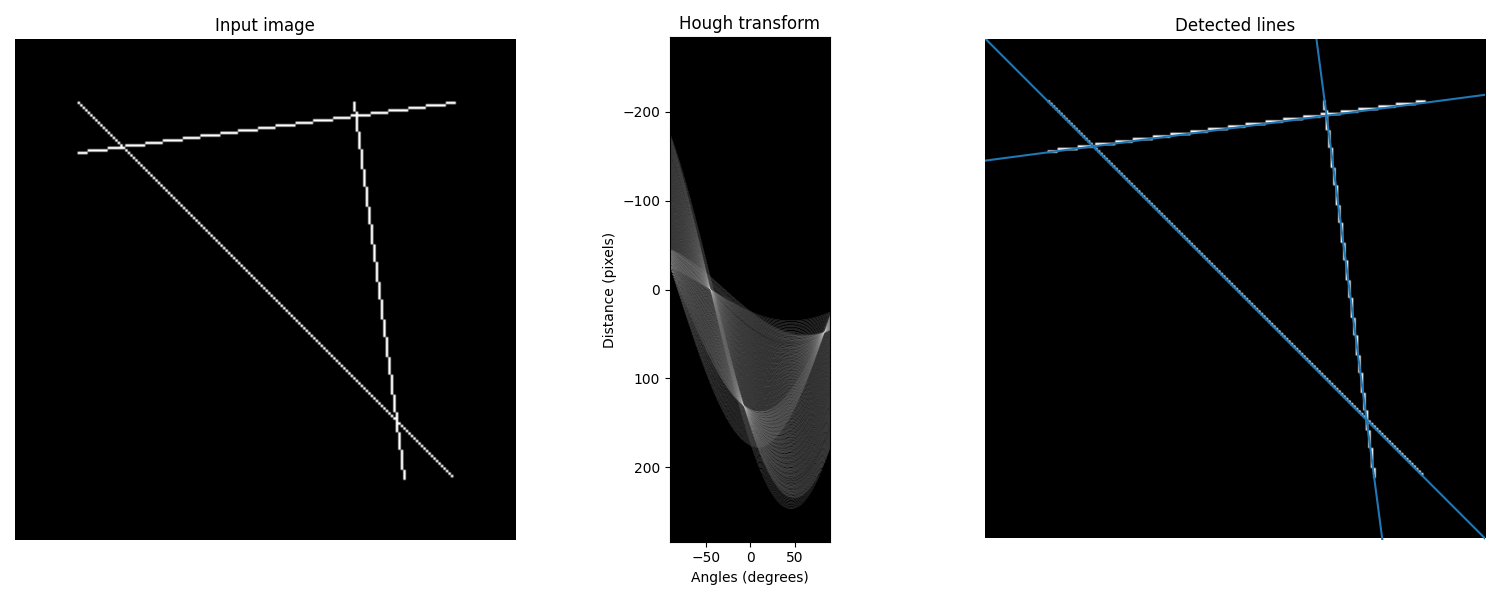
\includegraphics[width=0.5\linewidth]{figures/HoughTransform.png}
    \caption{Hough transform calculation to find the lines of a triangle \cite{hough}}
    \label{fig:houghl}
\end{figure}

\section{Image segmentation algorithms}
\label{sec:relatedsec1}

\subsection{Hough Transform}
\label{subsec:relatedsec1subsec1}

\par This technique was proposed by Paul Hough in 1962, as a method to identify patterns in images. \cite{Duda1972}
\par The Hough Transform is used in computer vision and image processing. The core idea behind it is a voting process made by the curves in the transform space, creating cluster points or local maxima. These points represent the existence of a shape, and since the curves contain the parameters of the shapes, from those parameters the position of the shape in the input image can be detected, like it is shown in Figure \ref{fig:houghl}.
\par The main strength of this method is that it is capable of identifying shapes even in slightly obscured or noisy data. This made this procedure a massive breakthrough in image processing. Since it's powerful to be able to detect shapes, the method is used in many sectors, from robotic navigation, by identifying edges and lines in the environment, to medical imaging, by detecting circular shapes potentially depicting different biological conditions and many more, where image processing can be utilized.

\subsection{Viola-Jones Face Detection}
\label{subsec:relatedsec1subsec2}
\par Another breakthrough in computer vision was the face detection procedure proposed by Paul Viola and Michael Jones in 2001. \cite{viola2001}
\par The main idea behind their approach lies in the usage of Haar-like feature and Adaptive Boosting.
\par The Haar-like features are simple rectangular regions in the input image data. The main goal of using these patterns is first to cut down on the necessary calculations by working with pixels, and second is to get a better understanding about certain regions in the image. By calculating the differences in the sum of pixel intensities between the regions, a contrast can be learned, an incredibly useful information which allows the detection of basic patterns, like edges, lines and textures.
\par Adaptive boosting is a machine learning algorithm used for boosting weak classifiers into a strong one. The main principle of this method is to iteratively  train weak classifier, each focusing on different features. At each iteration pass, the algorithm selects the best performing classifier and merges it with the final strong one, weight proportionally to its performance. It also weighs incorrectly classified instances more for the next iteration for the purpose of shifting the focus on the most challenging parts.
\par With the help of these two procedures the method of Viola and Jones achieves great accuracy in real-time, more specifically at 15 frames per second on a 700 MHZ Intel Pentium III, using approximately 50 thousand parameters. Since its low hardware requirements, this way of face detection is still used on very weak devices.

\section{Deep learning algorithms}
\label{sec:relatedsec2}
\par With the increase in computational power, image processing algorithms have also evolved in tandem. As seen in the Viola-Jones face detection algorithm, machine learning were already used in the early 2000s, be it at a smaller scale.
\par Since these algorithms now are able to utilize more resources, they can work with way more parameters, going from thousands to millions, allowing them to learn more complex features than before.
\par My choice for the following three deep learning architectures is that, they were significant achievements in the field of computer vision, while also resembling my chosen base model the MobilNet.

\subsection{YOLO}
\label{subsec:relatedsec2subsec1}
\par YOLO (You only live once) is an object detection method, based on a Convolutional Neural Network backbone, the building blocks of which can be seen in Table \ref{YoloTable}, containing convolutional layers of varying sizes.
\par The main selling point of this algorithm, is that it achieves real-time performance with a single-pass approach. It divides the image into a grid, each predicting a bounding box, with an associated confidance score and class probability. Utilizing these parameters and various anchor boxes, which are bounding boxes with a predefined shape, size and aspect ratio, the model predicts the final bounding box for the searched cell. \cite{redmon2018yolov3}
\par Since its real-time performance the method has been utilized in many projects, from autonomous driving, to surveillance systems.

\begin{table}[htbp]
\begin{center}
\begin{tabular}
{|p{90pt}|p{90pt}|p{90pt}|p{90pt}|}
\hline
 Type  &  Filters & Size & Output\\
\hline 
\hline Convolutional & $64-1024$ & $3x3/2$ & $128x128-8x8$ \\
\hline Convolutional & $32-512$ & $1x1$ & $ $ \\
\hline Convolutional & $64-1024$ & $3x3$ & $ $ \\
\hline Residual & $ $ & $ $ & $128x128-8x8$ \\
\hline
\end{tabular}
\end{center}
\caption{Building blocks for the YoloV3 CNN backbone, Darknet-53 \cite{redmon2018yolov3}}
\label{YoloTable}
\end{table}

\subsection{RESNET}
\label{subsec:relatedsec2subsec2}
\par ResNet is a convolutional neural network proposed by Kaiming He and co. in 2015, achieving great performances in various computer vision tasks.
\par The main strength of this model is that it addressed the vanishing gradient problem, via the introduction of skip connections. The residual blocks, the main building blocks of this model, contain the shortcut connections, skipping one or more layers. With this, the network is able to learn  residual functions, basically the difference between the desired output and the input data. This feature allows the ResNet architecture to increase the depth of the model, without the gradient vanishing. \cite{he2015deep}
\par As can be seen in Table \ref{ResNetTable}, the complexity of this model can grow to incredible levels, containing as much as 19.7 million parameters, meaning the number of calculation for one single pass through of this architecture is around that number.

\begin{table}[htbp]
\begin{center}
\begin{tabular}
{|p{120pt}|p{120pt}|}
\hline
Number of layers & Number of parameters\\
\hline 
\hline $20$ & $0.27M$ \\
\hline $32$ & $0.46M$ \\
\hline $44$ & $0.66M$ \\
\hline $56$ & $0.85M$ \\
\hline $110$ & $1.7M$ \\
\hline $1202$ & $19.7M$ \\
\hline
\end{tabular}
\end{center}
\caption{Correlation between the size of the model and the number of parameters used \cite{he2015deep}}
\label{ResNetTable}
\end{table}

\subsection{MOBILENET}
\label{subsec:relatedsec2subsec3}
\par MobileNet is a convolutional neural network designed specifically for mobile and other devices with limited computational power.

\begin{table}[htbp]
\begin{center}
\begin{tabular}
{|p{120pt}|p{120pt}|p{120pt}|}
\hline
Model & ImageNet Accuracy & Parameters\\
\hline 
\hline Conv MobileNet & $71.7\%$ & $29.3M$ \\
\hline MobileNet & $70.6\%$ & $4.2M$ \\
\hline
\end{tabular}
\end{center}
\caption{Difference in parameters between Depthwise separable and full convolutional MobileNet architecture \cite{howard2017mobilenets}}
\label{MobileNetTable}
\end{table}

\par At its core the architecture is built using depthwise separable convolutions. The standard convolutions is separated into two separated operations. The first one being a depthwise convolution, in which a single convolution filter is applied for each input channel, capturing features separatly. The second is pointwise operations, which applies a 1x1 filter to the outputs of the the previous calculations, combining the results. This allows the model to significantly reduce the number of parameters needed, compared to normal convolution, thus decreasing the computational power needed. \cite{howard2017mobilenets}
\par In Table \ref{MobileNetTable} the incredible difference between the complexity of the two architectures. For a 1.1 percent loss the exponential decrease in parameter count is a fantastic exchange.

%Adaugarea și Referirea la o Ecuație \ref{LabelMyEquation}.


 %\begin{equation}
 %    ws_N4 = w_{14}*N1 + W_{24}+N2 + w_{34}*N3
%\label{LabelMyEquation}
% \end{equation}

\chapter{Approaches for better performance with machine learning models}
\label{chap:preformance}

\par As the learning capabilities of deep neural networks increased over the years, so have their sizes in terms of the number of parameters and depth. With this the accuracy and speed of the models have increased, allowing for more and more use cases, like real-time predictions even on an everyday computer.
\par To be able to utilize a deep neural network algorithm in real-time, an architecture has to be chosen, which minimizes the number of parameters and overall size, while also maintaining a useful accuracy. There are a handful of such architectures, from which I will compare three.
\par For comparing the performance of the models, I am going to use the running time of one pass through the architecture in milliseconds. The goal is to use them in a real-time video processing application, with a reasonable frame rate of 24 frames per second, it means a running time needed of around 41 milliseconds. In practice this metric is dependent on a lot of variables, so it is not a hard requirement, just something to put the performances of the architectures in contrast.   

\section{Model comparisons}
\label{subsec:preformancesec1}

\subsection{Representative frames with deep learning}
\label{subsec:preformancesec1subsec1}

\par Starting with a simpler architecture in terms of the deep learning neural network, in the study of John and co. \cite{john2016} a high accuracy was achieved in real-time using representative frames, instead of a whole segment, with a specific algorithm, hence selecting better data for the machine learning model to predict from. Their algorithm clearly separated the two parts, the frame extraction running in  around 70 milliseconds and the classification running in around 40 milliseconds, achieving an accuracy of 91 percent.

\subsection{YOLOv3 performance}
\label{subsec:preformancesec1subsec2}

\par The YOLOv3 model is an efficient deep learning architecture, making it more than useful in achieving real-time performance on hand gesture detection and identification problems. In the approach of Mujahid, Awan and co. \cite{app11094164}, this algorithm was thought from scratch on the Mindst dataset \cite{deng2012mnist}, achieving good results. They proposed a lightweight architecture which is built on the YOLOv3 model, achieving impressive results, with an approximate accuracy rating of 98 percent in real-time, although time specifications were not provided.

\subsection{MobileNet performance}
\label{subsec:preformancesec1subsec3}

\par The approach of Wanga, Hua and Jina \cite{wang2021} consists of utilizing the architecture of MobileNet and Random Forest to identify hand gestures. They utilized the pretrained parameters of MobileNet on the ImageNet dataset \cite{deng2009imagenet}, than taking the output and running it through a Random Forest model to better extract features from the images. Their paper does not focus on performance in the context of the time needed for a prediction, that being said, since they use the MobileNet architecture as their backbone, which in a configuration of around 3.5 million parameters can achieve a pass-through time of around 35 milliseconds, from personal testing, it is safe to assume, that near real-time performance is achievable with their approach.
\par In Table \ref{MobileNetTable} the comparison of two MobileNet models, one with and one without a random forest ending, can be seen with regard to their accuracy ratings on three different hand based image datasets. From the results we can conclude that both architectures can achieve good accuracy. Combining that with the low hardware requirements of the model, we get a perfect combination for a usage in real-time applications.

\begin{table}[htbp]
\begin{center}
\begin{tabular}
{|p{90pt}|p{90pt}|p{90pt}|p{90pt}|}
\hline
Model & SLD Dataset Accuracy & SLGI Dataset Accuracy & Fingers Dataset Accuracy\\
\hline 
\hline MobileNet & $74.25\%$ & $94.12\%$ & $97.02\%$\\
\hline MobileNet-RF & $80.97\%$ & $95.12\%$ & $99.72\%$\\
\hline
\end{tabular}
\end{center}
\caption{MobileNet and MobileNet-RF accuracy, from the study of Wanga and co. \cite{wang2021}, on the Sign Language Digital Dataset (SLD) \cite{kopf:22025:sign-lang:lrec}, Sign Language Gestures Image Dataset (SLGI) \cite{jimaging9120262} and the Fingers Dataset}
\label{MobileNetTable}
\end{table}

\section{Transfer learning}
\label{subsec:preformancesec2}

\par Transfer learning is a machine learning technique where a pretrained model on a specific task and dataset is repurposed and fine-tuned for a different but similar problem. The pretrained values are taken for a new task, since the learned functions are usable in the new context, like in the example of identifying animals and human faces, the pretrained values will help to extract certain features which characterizes these objects, like facial line structures.
\par Using this method the deep neural network will start in closer to optimal position when learning features, jump starting the process, and enhancing the overall accuracy of the model. It is also a very useful tool, when dealing with a smaller dataset, or when collecting more data proves to be more challenging, allowing the architecture to learn with less data. This is also the reason why this approach is used in this application, since collecting thousands of images and labeling every one of them would take up an incredible amount of time.
\chapter{Machine learning model specifications}
\label{chap:model}

\par Creating and training a model from scratch requires a lot of resources in terms of hardware and data, even with smaller models in order to achieve high performance, so in order to ensure good results I will utilize transfer learning with a pretrained MobileNet architecture.

\section{MobileNet specifications}
\label{sec:modelsec1}

\par The used model is downloaded from the TensorFlow Model Garden \cite{modelGarden}, specifically the ssd-mobilenet-v2-fpnlite-320x320-coco version. The ssd, meaning single shot detector, is an architecture which uses the MobileNet model as its base. Fpn means feature map network, which is a method to extract information from multiple resolution levels in the image and perform the object detection on those. Coco is the name of the dataset on which the model is initially trained and the 320x320 means the image resolution for training.

\subsection{Model specifications}
\label{sec:modelsec1subsec1}

\par The architecture being a single shot detector means that one pass through is enough for predicting the objects and their bounding boxes \cite{ssd}.

\begin{figure}
    \centering
    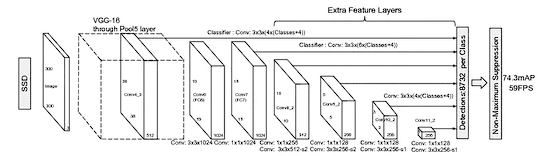
\includegraphics[width=0.5\linewidth]{figures/SSD.png}
    \caption{Architectural diagram of the SSD MobileNet model \cite{ssd}}
    \label{fig:ssd}
\end{figure}

\par In figure \ref{fig:ssd} we can see the overall architecture of a general ssd fpn model. In the case of this application the first few convolutional layers, the deep learning backbone, is replaced with the MobileNet architectures first few layer, which have been discussed in section \ref{subsec:relatedsec2subsec3}. The following few convolutional layers are the feature map network part. In this section the features processed by the machine learning model are made smaller and smaller, with every one of them having a connection to the prediction layer, hence enabling the architecture to learn with different ratios.
\par The predictions are done with help of 3x3xp kernels, where p is the number of channels in the feature map, which produce category scores or shape offsets for the bounding boxes. In the end filters are used at each cell in the feature maps to calculate 4 offsets relative to specified default bounding boxes \cite{ssd}.

\subsection{Original dataset}
\label{sec:modelsec1subsec2}

\par The model was pretrained on the COCO dataset, which contains around two hundred thousand labeled object in around 80 different categories, specifically made for the purposes of object detection by a team of researchers \cite{coco}.

\subsection{Model output}
\label{sec:modelsec1subsec3}

\par This architecture outputs a number of values regarding bounding boxes in raw and relative, value between 0 and 1, form and the predicted classes with their probabilities. In the case of the application three values are the most important: the class index, the prediction confidence and the relative bounding boxes. The confidence and index are needed for all hand gestures, while the box coordinate values are used when calculating the pixel positions for drawing.

\section{Data}
\label{sec:modelsec2}

\par In order to have creative freedom over the hand gestures, a custom dataset was made by me with five hand gestures and 20 pictures each. Some examples can be seen in figure \ref{customDataset}. The images than were labeled by hand with labelimg tool \cite{labelImg} and transformed into TF records, which is a specific format for the tensorflow object-detection api when teaching models with the script provided by them \cite{tfRecords}.

\begin{figure}
    \centering
    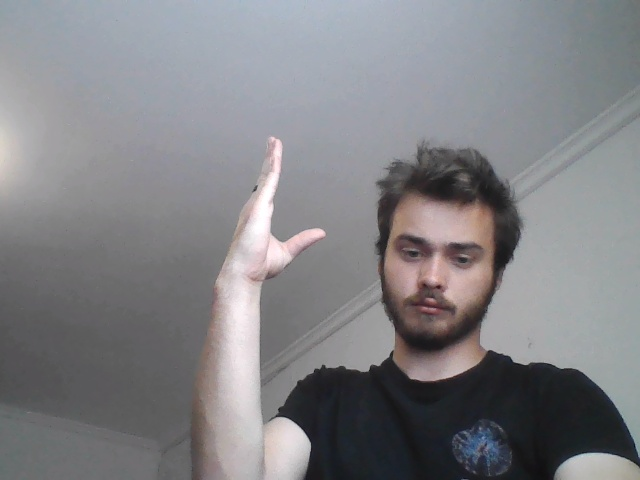
\includegraphics[width=0.22\linewidth]{figures/voiceup.jpg}
    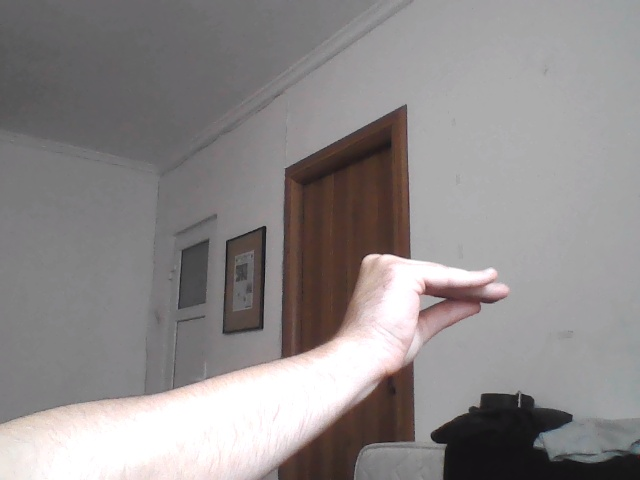
\includegraphics[width=0.22\linewidth]{figures/voicedown.jpg}
    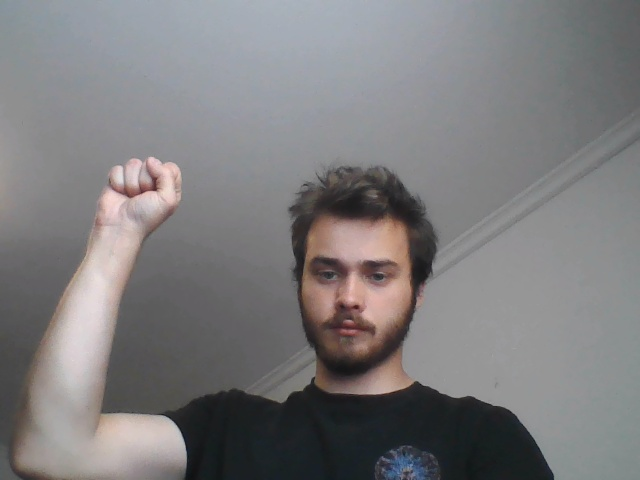
\includegraphics[width=0.22\linewidth]{figures/mute.jpg}
    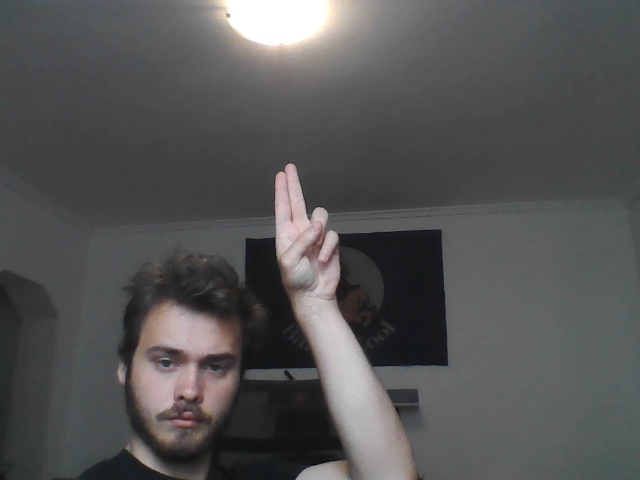
\includegraphics[width=0.22\linewidth]{figures/draw.jpg}
    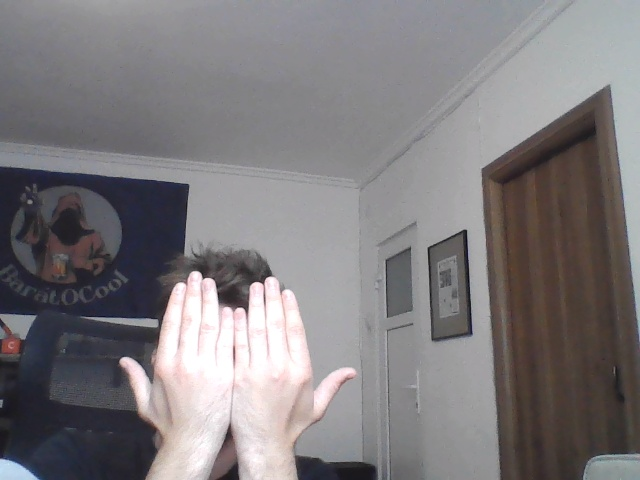
\includegraphics[width=0.22\linewidth]{figures/clear.jpg}
    \caption{Pictures for each functioning hand gesture in the dataset}
    \label{customDataset}
\end{figure}

\section{Training}
\label{sec:modelsec3}

\par The training of the model was done with the help of the provided script and configuration file by the tensorflow api \cite{trainingScript}. The configurations were personalized with the relevant paths to the label and record files and with the output path. The training was conducted with a batch size of 8 and 5 classes, decreasing learning rate and 20000 steps on an Nvidia 1660 Ti gpu.

\section{Metrics and running specifications}
\label{sec:modelsec4}

\par During training the learning rate slowly decreased in order to achieve a better approximations of the function as the model got closer to a local minimum, and the loss of the prediction have declined in a nice curve up until to a sufficient point, where it is low enough and the risk of over-fitting is not that high as can be seen in figure \ref{metrics}.

\begin{figure}
    \centering
    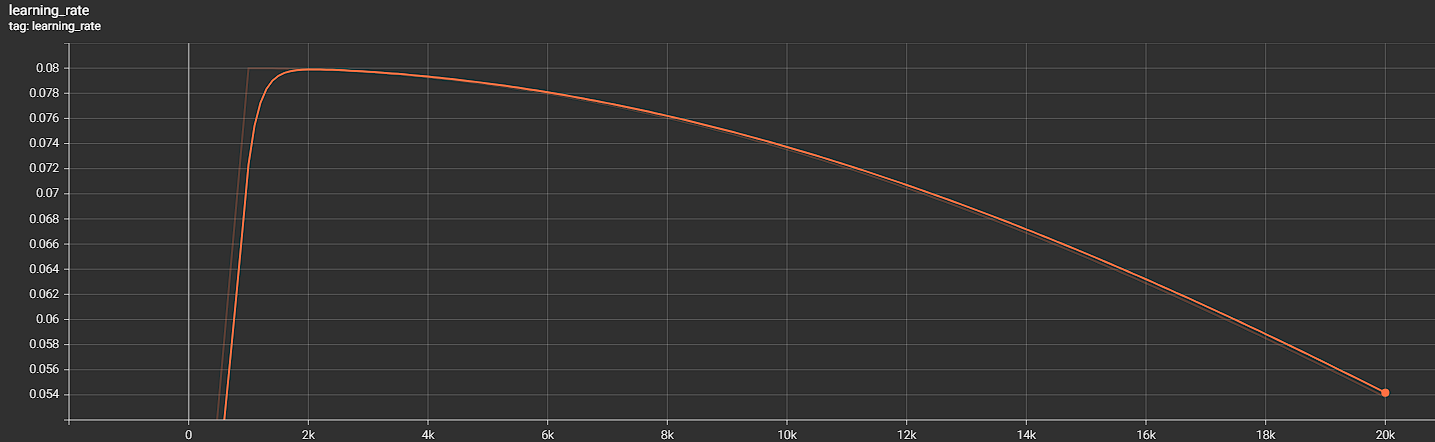
\includegraphics[width=0.4\linewidth]{figures/Learning-rate-graph.png}
    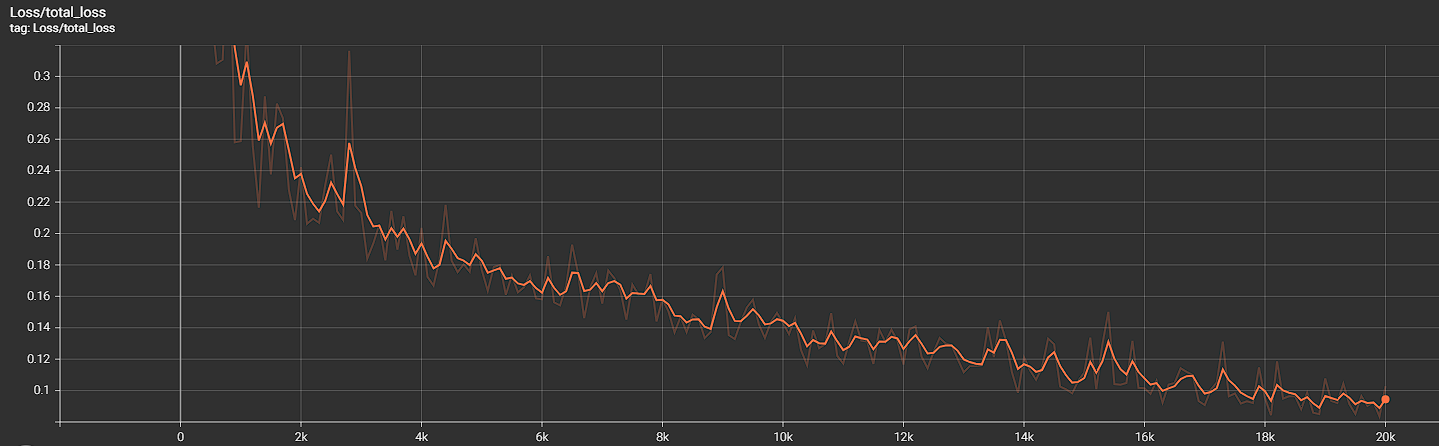
\includegraphics[width=0.4\linewidth]{figures/Loss-Graph.png}
    \caption{The changes of the learning rate and loss values throughout the training process}
    \label{metrics}
\end{figure}

\par As for the accuracy in real usage, the model can predict with around a 90 percent accuracy when the hand gesture features are visible. This means that the hands are not far enough from the camera, around 3 meters, that details can be barely visible, and an adequate light source is behind the camera.
\par For saving the application a script was provided by the api \cite{exportScript}, which exports the trained model in the format of the base tensorflow library, which makes the running of it easier in an application. To utilize the model the only thing that has to be done is to load it inside the application and add a batch layer to the image.
\chapter{Application requirements and specifications}
\label{chap:specs}

\par The main goal of the application is to create an alternative way of interacting with a live video. For this purpose a deep learning neural network is used, more precisely a MobileNet model pretrained on the ImageNet dataset, with custom final layers for identification. The machine learning algorithm will identify hand gestures, acting as the controlling tools for the application. 

\section{Application requirements}
\label{sec:specssec1}

\par The main focus of the application is the alternative way of interacting with the live video feed, providing feature for drawing with a finger, using simple hand gestures for clearing the drawings, for zooming in on a specific section of the video, for changing the volume of the recording and for taking a screenshot.
\par Besides the hand driven way of interactions the volume settings and the screenshot features all have a specific buttons and toggles, so they can be worked with normally with normal mouse actions.
\par The application can also be used as a simple video recording software, providing settings options for camera and microphone selection, changing the folder to which save the video files and screenshots.
\par All of the above is in visual format in the use case diagram below \ref{fig:usecase}, which was created by an online tool called Lucidchart \cite{lucidchart}.

\begin{figure}
    \centering
    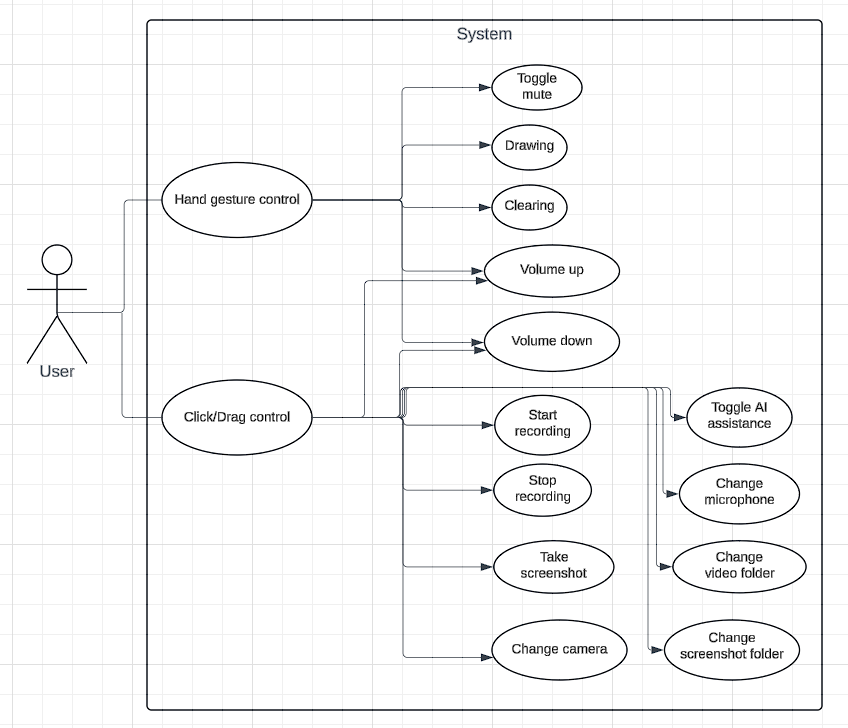
\includegraphics[width=0.8\linewidth]{figures/UseCaseDiagram.png}
    \caption{Use case diagram for the functionalities of the application}
    \label{fig:usecase}
\end{figure}

\subsection{Functional requirements}
\label{sec:specssec1subsec1}

\par To see the functionalities of the applications in an easier way, all of the above mentioned features are represented and described as use cases. The list with them is presented in Table\ref{UseCaseTable}, while the descriptions will be in the ones after.

\begin{table}[htbp]
\begin{center}
\begin{tabular}
{|p{90pt}|p{270pt}|}
\hline
 Use Case & Name\\
\hline 
\hline F1 & Start recording \\
\hline F2 & Stop recording \\
\hline F3 & Take screenshot \\
\hline F4 & Change volume up \\
\hline F5 & Change volume down \\
\hline F6 & Change video folder path \\
\hline F7 & Change screenshot folder path \\
\hline F8 & Change camera used during recording \\
\hline F9 & Change microphone used during recording \\
\hline F10 & Toggle artificial intelligence assistance \\
\hline F11 & Draw during recording \\
\hline F12 & Clear screen after drawing \\
\hline F13 & Toggle being muted \\
\hline F14 & Zoom in a portion of the video \\
\hline F15 & Zoom out \\
\hline
\end{tabular}
\end{center}
\caption{The application's functionalities represented as use cases}
\label{UseCaseTable}
\end{table}

\subsection{Functional requirements descriptions}
\label{sec:specssec1subsec1d1}

\par The F1 requirement is responsible for starting the video capture process. The steps and requirements for this functionality can be found in the table below \ref{F1Table}.
\par Prerequisites: The user chose a functioning camera and microphone; The user chose a path for the video to be saved in.
\par Post: The live feed of the video recording shows up on the screen; A pop-up error message is shown that the start was not successful.

\begin{table}[htbp]
\begin{center}
\begin{tabular}
{|p{180pt}|p{180pt}|}
\hline
 User & System\\
\hline 
\hline 1. The user presses the Start button &  \\
\hline  & 2. The system checks for a functioning camera and microphone \\
\hline  & 3. The system checks if the folder path given exists or not \\
\hline  & 4 The system starts the video capture \\
\hline  & 4.1 The system presents the live feed on the screen \\
\hline  & 4.2 The system shows a pop-up error message about the failure \\
\hline
\end{tabular}
\end{center}
\caption{F1 Functionality steps}
\label{F1Table}
\end{table}

\par The F2 requirement is responsible for stopping the video capture process. The steps and requirements for this functionality can be found in the table below \ref{F2Table}.
\par Prerequisites: The video recording is running successfully.
\par Post: The live feed on the screen will stop and turn into a black image and the video is present in the chosen folder; A pop-up message is shown about the failure of stopping the capturing.

\begin{table}[htbp]
\begin{center}
\begin{tabular}
{|p{180pt}|p{180pt}|}
\hline
 User & System\\
\hline 
\hline 1. The user presses the Stop button &  \\
\hline  & 2. The system stops the recording process \\
\hline  & 3. The system creates the final video file in the selected folder \\
\hline  & 3.1 A black image is shown instead of the live feed \\
\hline  & 3.2 The system shows a pop-up error message about the failure \\
\hline
\end{tabular}
\end{center}
\caption{F2 Functionality steps}
\label{F2Table}
\end{table}

\par The F3 requirement is responsible for taking a screenshot from the live feed. The steps and requirements for this functionality can be found in the table below \ref{F3Table}.
\par Prerequisites: The video recording is running successfully; A valid path is chosen as the screenshot folder.
\par Post: A pop-up message shows the screenshot was successfully taken and the picture will be present in the given folder; A pop-up error message is shown.

\begin{table}[htbp]
\begin{center}
\begin{tabular}
{|p{180pt}|p{180pt}|}
\hline
 User & System\\
\hline 
\hline 1. The user presses the Screenshot button &  \\
\hline  & 2. The system saves the last frame as an image in the chosen folder \\
\hline  & 3.1 A pop-up message is shown that the screenshot was taken successfully \\
\hline  & 3.2 The system shows a pop-up error message about the failure \\
\hline
\end{tabular}
\end{center}
\caption{F3 Functionality steps}
\label{F3Table}
\end{table}

\par The F4 requirement is responsible for changing the volume up. The steps and requirements for this functionality can be found in the table below \ref{F4Table}.
\par Prerequisites: The volume is not at 100 percent; For hand gesture control the recording is running and the AI assistance is turned on.
\par Post: The volume of the audio will be changed in the current or next recording.

\begin{table}[htbp]
\begin{center}
\begin{tabular}
{|p{180pt}|p{180pt}|}
\hline
 User & System\\
\hline 
\hline 1.1 The user moves the volume slider to the right &  \\
\hline 1.2 The user show a specific hand gesture &  \\
\hline  & 2. The system saves the volume modifier accordingly \\
\hline
\end{tabular}
\end{center}
\caption{F4 Functionality steps}
\label{F4Table}
\end{table}

\par The F5 requirement is responsible for changing the volume down. The steps and requirements for this functionality can be found in the table below \ref{F5Table}.
\par Prerequisites: The volume is not at 0 percent;For hand gesture control the recording is running and the AI assistance is turned on.
\par Post: The volume of the audio will be changed in the current or next recording.

\begin{table}[htbp]
\begin{center}
\begin{tabular}
{|p{180pt}|p{180pt}|}
\hline
 User & System\\
\hline 
\hline 1.1 The user moves the volume slider to the left &  \\
\hline 1.2 The user show a specific hand gesture &  \\
\hline  & 2. The system saves the volume modifier accordingly \\
\hline
\end{tabular}
\end{center}
\caption{F5 Functionality steps}
\label{F5Table}
\end{table}

\par The F6 requirement is responsible for changing the folder path for the video files. The steps and requirements for this functionality can be found in the table below \ref{F6Table}.
\par Prerequisites: The video recording is not running.
\par Post: The folder path for the video files will be changed accordingly and the user is sent back to the main window.

\begin{table}[htbp]
\begin{center}
\begin{tabular}
{|p{180pt}|p{180pt}|}
\hline
 User & System\\
\hline 
\hline 1. The user presses the Settings button &  \\
\hline  & 2. The current window is changed to the Settings window \\
\hline 3. The user presses the "Choose Path" button in the "Video folder path" section&  \\
\hline  & 4. The windows File explorer opens \\
\hline 5. The user chooses a folder &  \\
\hline  & 6. The system changes the path to the chosen one without saving it \\
\hline 7. The user presses the Save button &  \\
\hline  & 8. The system saves the setting changes to the configuration file \\
\hline  & 9. The system switches back to the main window \\
\hline
\end{tabular}
\end{center}
\caption{F6 Functionality steps}
\label{F6Table}
\end{table}

\par The F7 requirement is responsible for changing the folder path for the screenshots. The steps and requirements for this functionality can be found in the table below \ref{F7Table}.
\par Prerequisites: The video recording is not running.
\par Post: The folder path for the screenshots will be changed accordingly and the user is sent back to the main window.

\begin{table}[htbp]
\begin{center}
\begin{tabular}
{|p{180pt}|p{180pt}|}
\hline
 User & System\\
\hline 
\hline 1. The user presses the Settings button &  \\
\hline  & 2. The current window is changed to the Settings window \\
\hline 3. The user presses the "Choose Path" button in the "Screenshot folder path" section&  \\
\hline  & 4. The windows File explorer opens \\
\hline 5. The user chooses a folder &  \\
\hline  & 6. The system changes the path to the chosen one without saving it \\
\hline 7. The user presses the Save button &  \\
\hline  & 8. The system saves the setting changes to the configuration file \\
\hline  & 9. The system switches back to the main window \\
\hline
\end{tabular}
\end{center}
\caption{F7 Functionality steps}
\label{F7Table}
\end{table}

\par The F8 requirement is responsible for changing the used camera. The steps and requirements for this functionality can be found in the table below \ref{F8Table}.
\par Prerequisites: The video recording is not running.
\par Post: The chosen camera to be in use will be changed and the user is sent back to the main window.

\begin{table}[htbp]
\begin{center}
\begin{tabular}
{|p{180pt}|p{180pt}|}
\hline
 User & System\\
\hline 
\hline 1. The user presses the Settings button &  \\
\hline  & 2. The current window is changed to the Settings window \\
\hline 3. The user presses the drop-down list in the Camera section&  \\
\hline  & 4. The systems shows a list of available cameras \\
\hline 5. The user chooses a camera from the list &  \\
\hline  & 6. The system changes the camera to the chosen one without saving it \\
\hline 7. The user presses the Save button &  \\
\hline  & 8. The system saves the setting changes to the configuration file \\
\hline  & 9. The system switches back to the main window \\
\hline
\end{tabular}
\end{center}
\caption{F8 Functionality steps}
\label{F8Table}
\end{table}

\par The F9 requirement is responsible for changing the used microphone. The steps and requirements for this functionality can be found in the table below \ref{F9Table}.
\par Prerequisites: The video recording is not running.
\par Post: The chosen microphone to be in use will be changed and the user is sent back to the main window.

\begin{table}[htbp]
\begin{center}
\begin{tabular}
{|p{180pt}|p{180pt}|}
\hline
 User & System\\
\hline 
\hline 1. The user presses the Settings button &  \\
\hline  & 2. The current window is changed to the Settings window \\
\hline 3. The user presses the drop-down list in the Microphone section&  \\
\hline  & 4. The systems shows a list of available microphones \\
\hline 5. The user chooses a microphone from the list &  \\
\hline  & 6. The system changes the microphone to the chosen one without saving it \\
\hline 7. The user presses the Save button &  \\
\hline  & 8. The system saves the setting changes to the configuration file \\
\hline  & 9. The system switches back to the main window \\
\hline
\end{tabular}
\end{center}
\caption{F9 Functionality steps}
\label{F9Table}
\end{table}

\par The F10 requirement is responsible for toggling the AI assistance during video recording. The steps and requirements for this functionality can be found in the table below \ref{F10Table}.
\par Prerequisites: The video recording is not running.
\par Post: The AI assistance will be toggled on or off and the user is sent back to the main window.

\begin{table}[htbp]
\begin{center}
\begin{tabular}
{|p{180pt}|p{180pt}|}
\hline
 User & System\\
\hline 
\hline 1. The user presses the Settings button &  \\
\hline  & 2. The current window is changed to the Settings window \\
\hline 3. The user presses the toggle button in the "AI assistance" section  to change status&  \\
\hline  & 4. The system toggles the service on or off without saving the change \\
\hline 5. The user presses the Save button &  \\
\hline  & 6. The system saves the setting changes to the configuration file \\
\hline  & 7. The system switches back to the main window \\
\hline
\end{tabular}
\end{center}
\caption{F10 Functionality steps}
\label{F10Table}
\end{table}

\par The F11 requirement is responsible for hand driven drawing during video recording. The steps and requirements for this functionality can be found in the table below \ref{F11Table}.
\par Prerequisites: The video recording is running and the AI assistance is turned on.
\par Post: Given a specific hand gesture the system draws on the video feed following the users finger, visible both on the live feed and in the recording.

\begin{table}[htbp]
\begin{center}
\begin{tabular}
{|p{180pt}|p{180pt}|}
\hline
 User & System\\
\hline 
\hline 1. The user shows a specific hand gesture on the camera &  \\
\hline  & 2. The system whitens the pixels in a small radius near the finger of the user \\
\hline
\end{tabular}
\end{center}
\caption{F11 Functionality steps}
\label{F11Table}
\end{table}

\par The F12 requirement is responsible for clearing the video feed of any drawing during recording. The steps and requirements for this functionality can be found in the table below \ref{F12Table}.
\par Prerequisites: The video recording is running and the AI assistance is turned on.
\par Post: Given a specific hand gesture the system clears the video feed of any drawing.

\begin{table}[htbp]
\begin{center}
\begin{tabular}
{|p{180pt}|p{180pt}|}
\hline
 User & System\\
\hline 
\hline 1. The user shows a specific hand gesture on the camera &  \\
\hline  & 2. The system clears the video feed of any hand drawing \\
\hline
\end{tabular}
\end{center}
\caption{F12 Functionality steps}
\label{F12Table}
\end{table}

\par The F13 requirement is responsible for toggling being muted via hand gesture during video recording. The steps and requirements for this functionality can be found in the table below \ref{F13Table}.
\par Prerequisites: The video recording is running and the AI assistance is turned on.
\par Post: Given a specific hand gesture the system toggles between being muted and the previous audio level.

\begin{table}[htbp]
\begin{center}
\begin{tabular}
{|p{180pt}|p{180pt}|}
\hline
 User & System\\
\hline 
\hline 1. The user shows a specific hand gesture on the camera &  \\
\hline  & 2. The system toggles between being muted, audio level 0 percent and the previous level before the mute \\
\hline
\end{tabular}
\end{center}
\caption{F13 Functionality steps}
\label{F13Table}
\end{table}

\par The F14 requirement is responsible for zooming in a portion of the video controlled by a hand gesture. The steps and requirements for this functionality can be found in the table below \ref{F14Table}.
\par Prerequisites: The video recording is running and the AI assistance is turned on; The video feed is not zoomed in.
\par Post: Given a specific hand gesture the system zooms in a portion of the video where the users hand is.

\begin{table}[htbp]
\begin{center}
\begin{tabular}
{|p{180pt}|p{180pt}|}
\hline
 User & System\\
\hline 
\hline 1. The user shows a specific hand gesture on the camera &  \\
\hline  & 2. The system zooms in to the portion of the video where the users hand is present \\
\hline
\end{tabular}
\end{center}
\caption{F14 Functionality steps}
\label{F14Table}
\end{table}

\par The F15 requirement is responsible for zooming out of the zoomed in video feed. The steps and requirements for this functionality can be found in the table below \ref{F15Table}.
\par Prerequisites: The video recording is running and the AI assistance is turned on; The video feed is already zoomed in.
\par Post: Given a specific hand gesture the system zooms out, showing the full video.

\begin{table}[htbp]
\begin{center}
\begin{tabular}
{|p{180pt}|p{180pt}|}
\hline
 User & System\\
\hline 
\hline 1. The user shows a specific hand gesture on the camera in the zoomed in portion of the video &  \\
\hline  & 2. The system zooms out, showing the full video feed \\
\hline
\end{tabular}
\end{center}
\caption{F15 Functionality steps}
\label{F15Table}
\end{table}

\subsection{Non-functional requirements}
\label{sec:specssec1subsec2}

\par The application only has one version for the windows operating system, the results of running it on Linux, MacOS or any other operating system is undefined, they have not been test.
\par The processing of the input images from the video feed is done in real-time with the frame rate being determined by the input camera. The hand gesture identification and finger tracking is done on every second or third frame, depending on frame rate of the recording in the current moment.
\par The saving of the video files and images are done by only accessing those particular folders, with a naming convention of Recording\\Screenshot with the current date and time, so conflicts with other existing files is almost impossible, at the very least highly unlikely.

\subsection{System requirements}
\label{sec:specssec1subsec3}

\par The application only runs Windows operating system, needing the Windows 10 or 11 64-bit version, running on other versions may result in undefined behaviour.
\par In terms of the CPU the application was tested on Ryzen 7 4800h with a clock speed of 2.9 Gigahertz, from which 20-25 percent was used while running. From this data, an assumption can be drawn that as a baseline, a hardware similar to an intel core i7-9750h with a clock speed of 2.6 Gigahertz is advised. By having a weaker CPU the application may run into lagging issues when it comes to the rel-time performance of image processing.
\par The RAM used by the application is relatively small, using only 300 megabytes from a 3200 Megahertz unit.
\par In terms of storage, the application only needs around 300 Megabytes. The real impact will come from the saved video and screenshot files, depending on the file type in which they are saved.
\par To be able to use the application, the user also needs a working camera and a working microphone.

\label{sec:specssec2}

\section{Technical specifications}
\label{sec:specssec2}

\par For the purpose of easier integration of the deep learning model, the language used to develop the application is python, since most frameworks used for machine learning are written in this.
\par For creating and working with the MobileNet architecture, I use the TensorFlow \cite{tensorflow2015-whitepaper} and Keras framework \cite{chollet2015keras}. TensorFlow is an open-source project developed by Google giving an easy API for developing machine learning models efficiently, by wrapping up the more complex C++ and CUDA core functionalities. It also supports Keras, which is an open-source neural network library, providing an easy interface for building and teaching models, while also containing several known once, so they can be accessed with ease.
\par For the video capturing and the opencv library \cite{opencv_library}, which is open-source computer vision library written in mostly C++ and it is often used in machine learning projects. Because of that reason, the data, which is given back is easy to process and use in different models, making the development process that much easier.
\par Since the opencv library used for the capturing the visuals does not record audio as well, I use the pyaudio library, designed to capture the input of audio devices \cite{pyaudio}. This is a cross-platform python library published by the Massachusetts Institute of Technology for the purpose of recording and playing sounds. 
\par For the creation of the graphical user interface, the cross-platform Qt framework is used \cite{QtPage}. It is a wildly used service for creating high quality interfaces and is written in C++, providing good performance while supporting multiple languages like python. It provides various tools and modules, providing a relatively easy environment for UI development.
\par Besides the major libraries and framework, the win32api package \cite{win32api} is also used to access certain computer specifications, like the width and height of the monitor screen, to align the application at launch.
\par To store the settings of the user, the json format is used, so the structure of the storage is easy to read for both the application and the user, in case a manual change would be wanted. For this the built in json library \cite{jsonlib} is used in python.
\chapter{Application design and implementation}
\label{chap:design}

\section{Graphical User Interface}
\label{sec:designsec1}

\section{File Repository}
\label{sec:designsec2}

\section{Image processing}
\label{sec:designsec3}

\chapter{Application testing}
\label{chap:testing}

\section{Testing methods}
\label{sec:testingsec1}

\chapter{Future Work}
\label{chap:future}

\section{Machine Learning Model Improvements}
\label{sec:futuresec1}

\par The current model performs quite well in the ideal conditions stated in chapter \ref{chap:model}. Most of the shortcomings in other situations stem from the training data. In order to improve upon the model the dataset should be improved with approximately thousand of images, with different image conditions, including lighting, background distance and different obstacles, which takes some time, but is the next improvement step of the application.

\section{GPU Utilization}
\label{sec:futuresec2}

\par The tensorflow framework has built-in gpu utilization, however setting it up is independent of the application, because of the CUDA drivers. Another improvement is to try and achieve GPU utilization automatically, and looking into other types of GPU tools, since the current version only supports NVIDIA made graphics cards, which can run the 11.2 version of CUDA.

\chapter{Conclusions}
\label{conclusions}

\par In this this thesis I demonstrated that real-time hand gesture control with deep learning models, in order to provide, firstly, a convenient interaction with a live video feed and second, a drawing tool for better self expression, is possible locally on a mid-range machine.
\par I presented the the importance of deep learning models in the field of computer vision, while also exploring the performance metrics and shortcomings of different architectures, in order to find one which balances accuracy and quick runtime, ending up with the MobileNet model. After successfully finding a good model I went into the details of the applications, providing detailed descriptions about each functionality, while also providing hardware and software requirements. This continued with explained design choices describing the whole application and the solutions to some problems coming from some of the modules used. At the end some implementation details are provided with testing specifications.
\par With the constant rise of hardware, machine learning has become a very promising option for image processing. Even though most deep learning models are still too expensive to run on generic machines in real-time, hence most applications utilize massive servers and internet access, this thesis presents that the technology is now in a usable state for mass adoption even on local applications.
\par Even though this solution is not without its own problems, and it is not at the same level of accuracy as more advanced models, the machine learning and hardware sectors are in constant evolution, meaning the future, in terms of improvements, looks promising.
%\addcontentsline{toc}{chapter}{Concluzii}
%\addcontentsline{toc}{chapter}{Conclusions}

\bibliography{references}

\end{document}
